% Who introduced the method (or is it new)?
% Is your use of the method standard?
% Is your use of the method unusual?
% Are your methods mixed?

% Methods may involve: experiments, writing software, integrating software, proofs, case studies, observations/surveys, statistical analysis


\section{Methodology}

\subsection*{Task 1: propose a approach to form a unified knowledge graph to accommodate both user/item profile and interactions}

Here, we propose to form a heterogeneous knowledge graph that accommodate item/user profile information besides interactions records. We explore the semantic information of the graph structure to improve the data density, when interaction alone being too sparse to use. 

Firstly, we use side information to crate a knowledge graph. The knowledge graph node can either be item or important feature entities based on data exploration and analytics. Same process applies to the user side, i.e. profile information. In the end, we would have 2 heterogeneous knowledge graph, based on users and items perspectively. Illustrated as G1 and G2 in Fig \ref{fig:ikgraph}.

\begin{figure*}[!t]
    \centering
    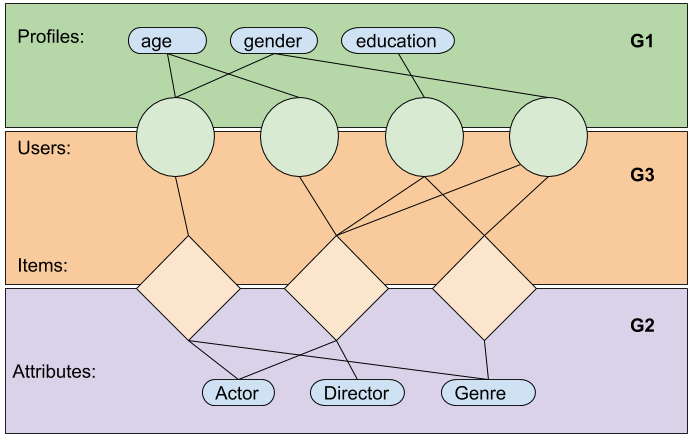
\includegraphics[width=0.8\textwidth]{figs/ikdiagram.png}
    \caption{G1:user knowledge graph, G2:item knowledge graph, G3:user-item bipartite graph}\label{fig:ikgraph}
\end{figure*}

Next we treat user-item interactions as a bipartite graph, as G3 in Fig \ref{fig:ikgraph}. This way user and item nodes in G1 and G2 are now connected with G3 via "interaction" edges. After this step, we get a unified heterogeneous knowledge graph which contains both user/item feature information as well as interactions.

As a result, such heterogeneous graph structure is open and capable of establish connections to new incoming data points. This leads to adaptiveness when handling cold start problem, which we will cover in task 3.


\subsection*{Task 2: Propose a method to leverage user/item representation with heterogeneous knowledge graph}


\begin{figure*}[!t]
    \centering
    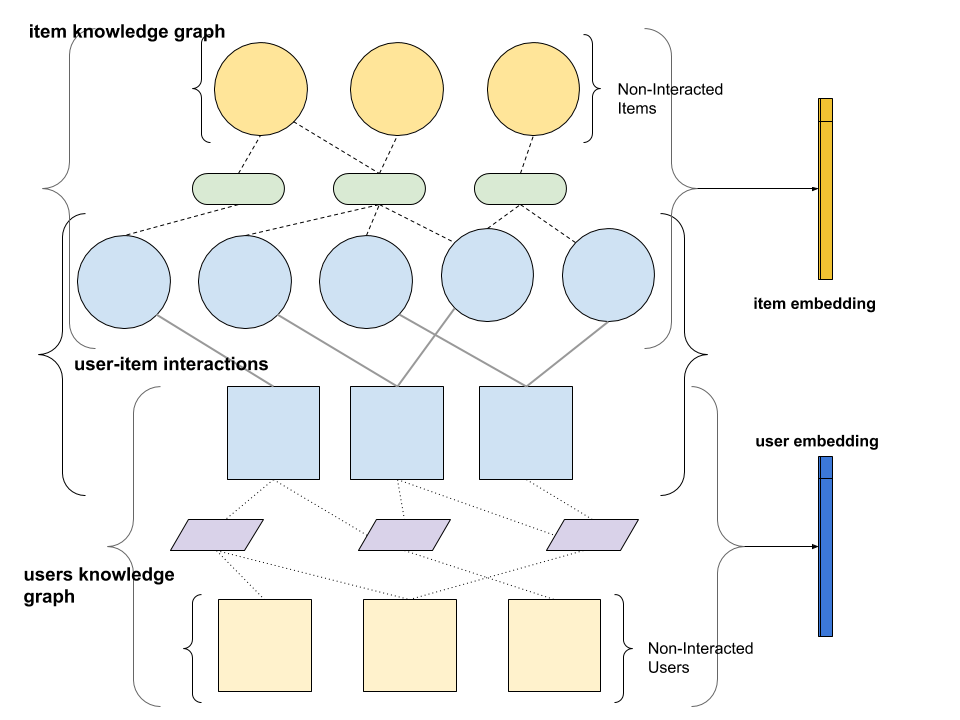
\includegraphics[width=0.8\textwidth]{figs/meta-embedding.png}
    \caption{meta-path based interactions via heterogeneous knowledge graph}\label{fig:meta_task2}
\end{figure*}

Following to Task 1, Incorporating the rich heterogeneous knowledge graph into recommender system is not straight forward. Most recommender models are only capable of processing structured data. The aim of this task is to transforming node into latent representation through nodes' neighborhood propagation for recommender system to use.

In addition to using direct connections, in this task, we adopts experts knowledge into representation modeling process by defining meta-path connections between nodes. Adopting expert knowledge brings a number of benefits:

Firstly, We establish indirect user-item relationship from the heterogeneous knowledge graph from task 1. For example, \textit{User - Movie} interaction, can be extend to \textit{User - Movie1 - Actor - Movie2}. As a result, collaborative filtering (CF) based recommendation approach can benefits from the denser interaction datasets. 

Subsequently, high-order connectivity with in heterogeneous knowledge graph is included as part of node representation learning process. So that, side information such as user demographics, item feature representation and node structural information can be learnt and transform into feature vectors for the representative model. 

Another added benefit of meta-path approach is reducing bias. Since, it happens commonly in early stage of recommender systems. i.e. When there is insufficient data available to represent a complete user/item distribution. 

Lastly, we propose a recommendation framework that incorporates above representation approach. By leverage CF information and path-based similarity within the heterogeneous knowledge graph. As illustrated in Fig \ref{fig:meta_task2}, both interacted and non-interacted user/item entities now can participated into recommender model training.

\subsection*{Task 3: to build a recommendation method that is adaptive to unseen data points}

So far in Task 1 and Task 2 try to alleviate data sparsity problem by forming heterogeneous knowledge and establish indirect connections via meta-path. However, our recommendation model is limited to a static dataset. i.e. The model is only capable of making predictions on data presented during training phase. 

The graph convolutional network based embedding approach had shown promising results on classification and link prediction problems. Inspired by GraphSAGE \citep{hamilton2017inductive} and graph attention network (GAT) \citep{velivckovic2017graph}, which introduced a general inductive framework to efficiently generate node embeddings for previously unseen data. \citet{hamilton2017inductive} uses function that generates embeddings by sampling and aggregating features from node neighbors.

In this task, we adopt the inductive approach above onto heterogeneous knowledge graph. In order to to extend model prediction capability, we need to work on 2 major parts: message propagation ability and aggregation rules through nodes neighborhood and layers. 
Following previous tasks, we apply GAT attention mechanism as part of the message propagation method via node neighborhood linkage and pre-defined meta-path connections. One side benefit of such approach is, expert define relationships can now be explained through attention weights, which leads to better model interpretability.
Next, we define appropriate aggregator approach from the node neighborhood. We measure and compare different pooling rules and attention mechanism for the inductive learning step.

Lastly, we evaluate the inductively generated node representation effectiveness by applying it in recommendation problem settings. 

At a high level, this task solves the limitations by incorporating graph structure and node attributes and generate node embeddings that were not present during training for recommendation predictions.


\subsection*{Task 4: Develop a knowledge transfer method to improve target domain data sparsity by leveraging source knowledge graph }

In tasks 1-3, we are focusing on 2 major challenge: 1. how to included data that lacks of interactions for training. 2. how to make predictions on data that emerged post training phase. In this task, we are going to focus more on transferring learnt knowledge from a different domain via knowledge graph to overcome the data sparsity problems.

First, we use common metadata (such as, item labels, demographics, etc.), to establish connections between source domain and target domain. 
Next, we propose a novel network transfer learning framework that leverage  adversarial domain adaptation technique and network multi-order interactions to enable knowledge transfer in a unified end-to-end framework. 

\subsection*{Task 5: Develop a multi-domains recommender systems based on heterogeneous knowledge graph}

\subsubsection*{Step 1: Define a unified optimization objective for knowledge graph based recommender system}
In this task, we aim to optimize node representation inside knowledge graph as well as collaborative user-item interactions recommendation in a jointly fashion.
Based on the findings from task 1-4, we apply earlier defined propagation rule and aggregator method under following objective function as:

\begin{equation}
    Target=\min{(L_\text{KGE}+L_\text{FM}+\lambda\|\theta\|^2_2)}
\end{equation}

Where $L_\text{KGE}$ is the optimization target for representation embedding in knowledge graph. Here we will experiment on different loss option for optimizing recommendation problem. For example, the entity relationship can be optimise based on translation principle \citep{lin2017learning}. 

\begin{equation}
    L_\text{KGE}=\sum{(h,r,t^+,t^-)} -ln_{sigmoid}(g(h,r,t^-)-g(h,r,t^+))
\end{equation}

While $g(h,r,t)$ is the projected probability from entity $h$ to target entity $t$ propagated via relationship $r$. $^+,^-$ stands for positive and negative samples. Accordingly $L_\text{FM}$ is the BPR \citep{rendle2012bpr} loss for optimizing recommendation objectives. 
\begin{equation}
    L_\text{FM}=\sum{(u,i^+,i^-) \in G_{u,i}} -ln_{sigmoid}(y(u,i^+)-y(u,i^-))
\end{equation}
Where y(u,i) commonly stands for user-item dot product, Intuitively, the its result can be regarded as similarity score.

Lastly, regularization is applied on $\theta$ as model parameters.

Consequently, the trained model entity representation would tailored toward the recommendation objective.


\subsubsection*{Step 2: Design a cross domains recommendation framework via knowledge graph}

In the second step, we extend recommendation model from single domain in Step 1 to multiple domains for further exploration on domain adaptation ability across multiple knowledge graphs.

Similarly to single domain, we extend user-item interactions across 2 different domains. Further side information as described in task 4 is serving as extra connections between target and source knowledge graphs.

Following GANs intuition, we introduce domain classifier D as critic, a binary classifier, to predict if positive sample item comes from source or target domain based on its representation. Intuitively, cross graphs node representation and D can be regarded as 2 player minimax game. It is expected node representation become domain-invariant when reaching equilibrium, i.e. knowledge is transfers across domains, that leads the source and target domain to be aligned. The domain alignment loss can be defined as:

\begin{equation}
    L_\text{DA}(e_s,e_t)=E_{e \in D_s}[log(1-D(e_s))] + E_{e \in D_t}[log(D(e_t))]
\end{equation}

Finally we adjust our cross domains recommendation objective to as following:

\begin{equation}
    Target=\min{(L_\text{DA}+L_\text{FM}+\lambda\|\theta\|^2_2)}
\end{equation}

\subsection*{Task 6:  A case study for validating the proposed recommendation approaches}

The research will be verified from two aspects: 
First, verify knowledge graph based recommendation approach using public datasets, such as DBLP DBLP Citation Networks, MovieLens data sets (http://www.grouplens.org/node/73). Similarity measure as well as adaptiveness are the core parts of this research, each aspects will be verified accordingly.

Second, the approach will be used in a real world data sets. Industries problems such as tourism and real estate listings which faces constant cold start problems will be used to further test the effectiveness of the proposed method.

